Для верификации вычислений приложения использовались статьи написанные по реальным экспериментальным данным полученных от коллабора-ции \textit{ATLAS}. Верифиционными данными являются ограничения на эффекты $Z$-${Z}^{\prime}$ смешивания на Большом Адронном колайдере.

Изучение процесса рождения ${W}^{+}{W}^{-}$ бозонной пары на Большом адронном коллайдере позволяет исследовать спонтанное нарушение калибровочной симметрии стандартной модели (\textit{SM}) и может использоваться для поиска новых явлений за пределами \textit{SM}. Дополнительные нейтральные векторные ${Z}^{\prime}$-бозоны, распадающиеся на заряженные калибровочные векторные пары бозонов ${W}^{+}{W}^{-}$, предсказаны во многих сценариях новой физики, включая модели с расширенным калибровочным сектором. Процесс $pp \rightarrow {W}^{+}{W}^{-}$  позволяет установить жесткие ограничения на угол смешивания $\xi$ для $Z$-${Z}^{\prime}$ и массу ${Z}^{\prime}$, ${M}_{{Z}^{\prime}}$. В настоящей работе впервые получены ограничения на параметры ${Z}^{\prime}$ смешивания в плоскости $\xi$–${M}_{{Z}^{\prime}}$, полученные из экспериментальных данных \textit{ATLAS} и \textit{CMS} на \textit{LHC} при энергии 13 ТэВ и светимостями 36,1 и 35,9 фб${}^{−1}$, соответственно. Область исключения была значительно расширена по сравнению с полученной из предыдущего анализа, выполненного с данными \textit{Tevatron}, а также с данными \textit{LHC}, собранными при 7 и 8 ТэВ. Полученные ограничения~\cite{2part-pankov} на угол смешивания $Z$-${Z}^{\prime}$ существенно превосходят ограничения, ранее полученные из глобального анализа электрослабых данных.

Многие новые физические сценарии (\textit{NP}) за пределами \textit{SM}, включая суперструнные и лево-симметричные модели, предсказывают существование новых нейтральных и заряженных калибровочных бозонов, которые могут быть достаточно легкими, чтобы быть доступными на текущих и / или будущих коллайдерах. Поиск этих новых нейтральных ${Z}^{\prime}$ и заряженных ${W}^{\prime}$ калибровочных бозонов является важным аспектом экспериментальной программы физики высокоэнергетических коллайдеров. Здесь рассматриваются  эффекты ${Z}^{\prime}$-бозонов. Существующие ограничения на прямое рождение на \textit{LHC} и виртуальные эффекты на Большом электронно-позитронном коллайдере (\textit{LEP}) путем интерференции или смешения с $Z$-бозоном подразумевают, что любой новый ${Z}^{\prime}$-бозон довольно тяжелый и очень мало смешивается с $Z$-бозоном. В зависимости от рассматриваемой теоретической модели массы ${Z}^{\prime}$ порядка 4,5 ТэВ и углы смешивания $Z$-${Z}^{\prime}$ на уровне нескольких промилле исключены. Угол смешивания сильно ограничен очень высокоточными экспериментами на \textit{LEP} и линейным коллайдером \textit{SLAC} (\textit{SLC}).

\begin{figure}[!h]
	\centering
	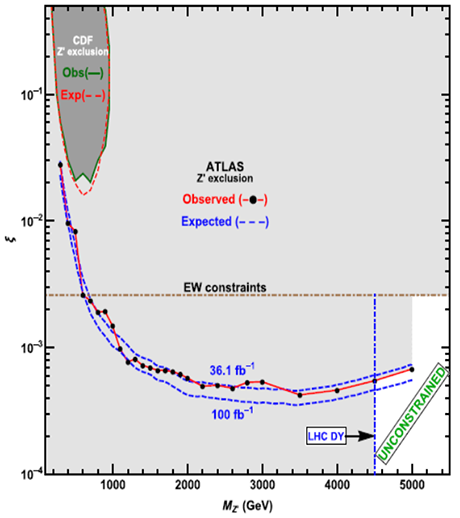
\includegraphics[width=\textwidth]{figures/verify-1.png}
	\caption{Ограничения на угол смешивания $Z$-${Z}^{\prime}$ полученные из обработки данных эксперимента \textit{ATLAS}}
	\label{fig:verify-1}
\end{figure}

\begin{figure}[!h]
	\centering
	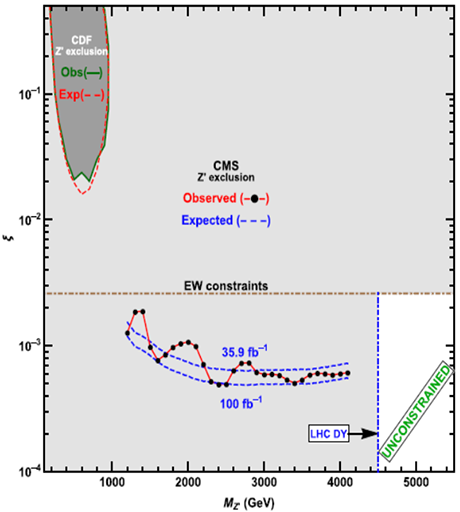
\includegraphics[width=\textwidth]{figures/verify-2.png}
	\caption{Ограничения на угол смешивания $Z$-${Z}^{\prime}$ полученные из обработки данных эксперимента \textit{CMS}}
	\label{fig:verify-2}
\end{figure}

Более подробно детали анализа данных экспериментов \textit{ATLAS} и \textit{CMS} представлены в работе~\cite{2part-pankov}. В результате обработки данных по измерению процесса рождения ${W}^{+}{W}^{-}$ пар в протон-протонных столкновениях получены экспериментальные ограничения на угол смешивания ${Z}^{\prime}$-бозонов в модели \textit{SSM}, которые составили $\xi$ < 0,0004 (рис.~\ref{fig:verify-1}, рис.~\ref{fig:verify-2}), что на порядок лучше результатов полученных ранее из глобального анализа электрослабых данных.